\addcontentsline{toc}{chapter}{PhD Activities}
\section*{PhD Activities}

This PhD thesis forms part of the research output of the NEMUS project, which focuses on the digital restoration of ancient musical instruments through physical modelling techniques. Part of the remit of NEMUS is the creation of digital musical instrument interfaces to numerical simulations of historical instruments. These interfaces aim to incorporate the tactile-kinaesthetic (``haptic'') feedback provided by the physical instrument being simulated. This work focused on the development of such an interface, particularly a seventeenth-century two-register harpsichord in the Italian style. NEMUS's dedication to open-sourcing its research outputs also led to the creation of the interface using entirely open-source hardware and software. As part of this, research tools with uses beyond the scope of NEMUS were identified for development and distribution under open-source licenses. One tool was chosen for further development due to its potential use within musical instrument conservation and was developed following an open-source methodology.

The first year focused on gathering and studying relevant literature, particularly concerning the creation of haptic interfaces. In addition to the literature review, research and prototyping tests were conducted to create the interface. A small-scale three-key mechanical model was purchased, and a selection of sensors was tested on it to identify a suitable candidate for the final interface. As part of the process, two institutes were identified for external collaboration and support. The first was San Colombano in Bologna, for its extensive harpsichord collection and the expertise of its staff in the field of historical Italian harpsichords. The second institute was Imperial College London, for its prolific research output in the field of digital musical instrument interfaces. After visits to both institutes, support was brokered between the curator of San Colombano, Catalina Vicens, and Professor Andrew McPherson, Chair in Design Engineering and Music at Imperial College London. A mechanical interface was commissioned from the luthier Roberto Livi, which was designed and created concurrently with the optical sensor system.

In the second year, the design and fabrication of the optical sensor system for the interface were carried out. This involved the fabrication of printed circuit boards, which were ordered from PCBWay. Given lead times, several designs were ordered simultaneously, each assembled and tested, with the most viable designs iterated upon for the next version. Part of this process required the furnishing of the NEMUS laboratory with appropriate equipment for PCB assembly and testing. Digital fabrication facilities for 3D-printed brackets and rigs were researched and identified within the Alma Labor facility at Unibo, managed by Massimiliano Fraulini. The first full interface was delivered in June of the second year, and all components were assembled and installed by October. Installation required multiple iterations of firmware as well as the creation of documentation for remote support and further refinement. This first model was installed for exhibition at San Colombano the following year.

Concurrent to the interface project, development was carried out on what would become known as the \textsc{magpie} framework—an open-source tool for thin-plate modelling and simulation using elastic boundary conditions. The framework was authored in both M\textsc{atlab} and the Python programming languages. The Python version was published to the Python Package Index in May 2024 for demonstration at the \href{https://cism.it/en/activities/courses/C2404/}{``Physics of Musical Instruments Applied to Instrument Making''} advanced course at the International Centre for Mechanical Sciences in Udine. A developed version of the framework with a graphical interface was accepted for presentation at the INTER-NOISE 2024 conference.

From June 2024, a year-long research visit to the University of Edinburgh was undertaken as part of the Una Europa Cultural Heritage doctorate. The Una Europa co-supervisor selected was Dr.\ Jenny Nex, curator of the musical instrument collection, who provided guidance and support within research on digital cultural heritage and musical instrument restoration. Additional guidance was provided by Jonathan Santa Maria Bouquet, Senior Conservator of the Heritage Collections of the University of Edinburgh, on materials and processes for the computer-aided manufacture of harpsichord parts. In addition to a further literature review, the visit provided the opportunity to consult the Edinburgh Futures Institute's Centre for Data Science and Culture and the Software Sustainability Institute to assess the open-source practices of the project. Part of this research included attendance at the \href{https://www.eventbrite.co.uk/e/the-digital-museum-conference-tickets-995019448957?aff=eemailordconf&utm_campaign=order_confirm&ref=eemailordconf&utm_medium=email&utm_source=eventbrite&utm_term=viewevent}{``Digital Museum Conference''} to learn more about the challenges facing museums and heritage institutions in incorporating digital technology.

Research carried out at Edinburgh informed the second iteration of the sensor system, which was presented as part of a paper at Forum Acusticum 2025 in Málaga, Spain. Research at the University of Edinburgh also led to the participation of the San Colombano exhibition as part of the Una Europa workshop on ``Museums and New Challenges: Virtual Technologies, Social Responsibility and Environmental Sustainability.'' The final year saw the completion of the second interface and the presentation of the first at the NIME 2025 conference in Canberra, Australia.

\clearpage

% 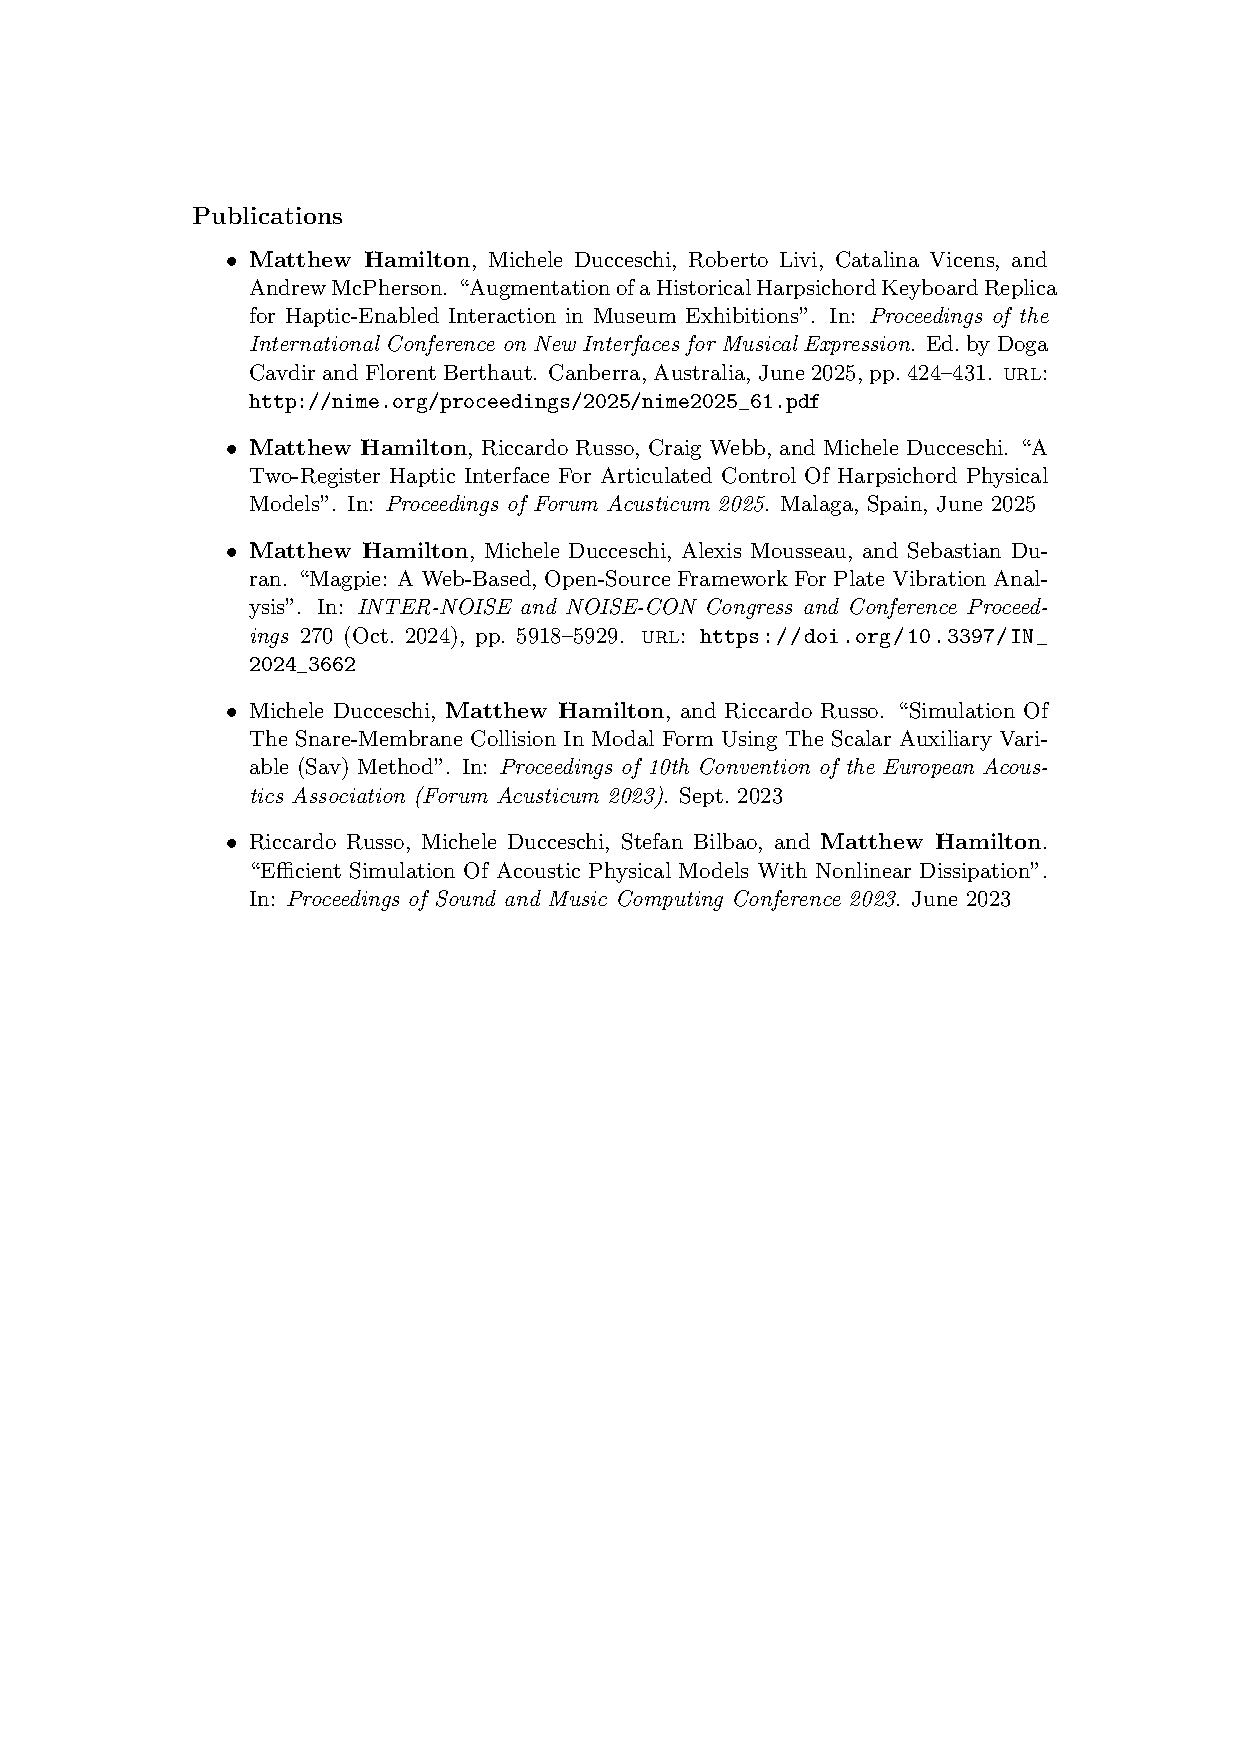
\includepdf[
%       pages = -,
% pagecommand = {\thispagestyle{headings}}
% ]{front_matter/publications.pdf}

\subsection*{Publications}
\begin{refsection}
\begin{itemize}
    \item \fullcite{hamilton_augmentation_2025_activities}
    \item \fullcite{hamilton_two_2025_activities}
    \item \fullcite{hamilton_magpie_2024_activities}
    \item \fullcite{ducceschi_simulation_2023_activities}
    \item \fullcite{russo_efficient_2023_activities}
\end{itemize}
\end{refsection}